\chapter{Model grafowy problemu zakupu licencji}

\section{Reprezentacja grafowa}

\paragraph{Konwencje terminologiczne} W pracy słowo „licencja grupowa” oznacza typ umożliwiający współdzielenie dostępu przez właściciela oraz jego sąsiadów w grafie (wyłącznie sąsiedztwo bezpośrednie). „Pojemność” oznacza całkowity rozmiar grupy wraz z właścicielem (min–max). Dla czytelności stosujemy skróty nazw modeli: Erdős–Rényi (ER), Watts–Strogatz (WS), Barabási–Albert (BA).

Aby formalnie opisać zjawisko współdzielenia licencji, sieć relacji społecznych modelujemy jako graf nieskierowany \( G = (V, E) \). Każdy wierzchołek \( v \in V \) reprezentuje pojedynczego użytkownika, natomiast krawędź \( \{u, v\} \in E \) oznacza, że użytkownicy \( u \) i \( v \) znajdują się w relacji umożliwiającej współdzielenie licencji - na przykład jako znajomi lub członkowie rodziny. Graf jest nieskierowany, ponieważ zakładamy symetryczność tej relacji: jeśli \( u \) zna \( v \), to również \( v \) zna \( u \).

Przyjmujemy również, że graf \( G \) nie zawiera pętli, tj. \( \{v, v\} \notin E \) dla każdego \( v \in V \), ani krawędzi wielokrotnych - każda para użytkowników może być powiązana co najwyżej jedną krawędzią. Przykład takiej struktury zilustrowano na Rysunku \ref{fig:social_graph}.

\begin{figure}[H]
    \centering
    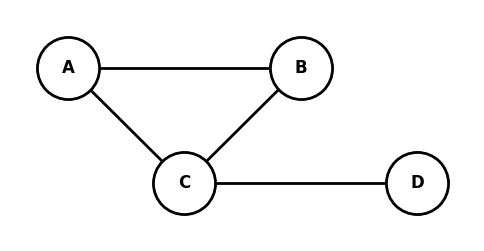
\includegraphics[width=0.5\textwidth]{assets/graphmodelexample.png}
    \caption{Przykładowy graf relacji społecznych między użytkownikami.}
    \label{fig:social_graph}
\end{figure}

\paragraph{Przykład (ilustracja doboru grup).} Rozważmy graf z rys.\,\ref{fig:social_graph} i konfigurację \texttt{duolingo\_super} (\emph{Individual} 1–1, \emph{Family} 2–6). Jeśli węzeł $u$ ma czterech sąsiadów i wszyscy są wzajemnie niepołączeni, opłaca się utworzyć grupę rodzinną o rozmiarze 5 (właściciel + 4 członków). Gdyby zaś sąsiedzi tworzyli gęstą klikę i pojawiały się konflikty (np. ograniczone możliwości pojemności u różnych właścicieli), heurystyki preferujące \emph{unikalne pokrycie} będą wybierały kilku właścicieli o mniejszych grupach. Takie scenariusze omówiono na rysunkach w rozdz.\,\ref{chap:algorithms} oraz w części eksperymentalnej.

Opisana reprezentacja, w której wierzchołki odpowiadają jednostkom, a krawędzie bezpośrednim relacjom umożliwiającym interakcję, jest powszechnie stosowana w analizie sieci społecznościowych \cite{Brandes2004, NETTLETON20131}. Takie ujęcie pozwala formalnie modelować i badać zjawiska zachodzące w społecznościach użytkowników usług cyfrowych.

W przyjętym modelu zakłada się, że współdzielenie licencji może odbywać się wyłącznie między osobami połączonymi bezpośrednią krawędzią w grafie. Oznacza to, że użytkownicy muszą znać się bezpośrednio i mieć wzajemne zaufanie, co jest istotne na przykład w przypadku przekazywania danych logowania lub zapraszania do planu rodzinnego. Relacje pośrednie, w których użytkownicy są powiązani poprzez wspólnych znajomych (np. \( A \sim B \) oraz \( B \sim C \), lecz brak bezpośredniego powiązania \( A \sim C \)), nie są uwzględniane w analizie. Oznacza to, że dla danego grafu \( G = (V, E) \),
w którym \( V \) to zbiór użytkowników, a \( E \subseteq \{ \{u,v\} : u,v \in V, u \neq v \} \) to zbiór relacji znajomości, analizie podlegają wyłącznie relacje bezpośrednie, czyli pary \( \{u, v\} \in E \).
Na przykład w grafie przedstawionym na Rysunku \ref{fig:social_graph}, użytkownicy \( A \) i \( D \) są wprawdzie połączeni za pośrednictwem ścieżki \( A \rightarrow C \rightarrow D \), jednak ponieważ brakuje bezpośredniego połączenia \( \{A,D\} \in E \), to taka relacja nie jest uznawana za podstawę do współdzielenia licencji w tym modelu.
Mimo że w praktyce relacje pośrednie - takie jak ścieżki długości większej niż jeden - mogą sprzyjać tworzeniu grup subskrypcyjnych, w analizie zostały one pominięte w celu uproszczenia problemu.

Graf społecznościowy nie musi być pełny - dopuszcza się dowolną strukturę odpowiadającą rzeczywistym relacjom społecznym. W analizie istotną rolę odgrywa stopień wierzchołków, ponieważ decyduje on o liczbie osób, którym dany użytkownik może udostępnić swoją licencję. Dla wierzchołka \( v \in V \), jego stopień oznaczamy przez \( \deg(v) \), co odpowiada liczbie sąsiadów użytkownika \( v \) w grafie \( G = (V, E) \).

Należy jednak zauważyć, że nawet w przypadku wysokiego stopnia \( \deg(v) \), użytkownik niekoniecznie może współdzielić licencję ze wszystkimi swoimi sąsiadami. Ograniczenia techniczne, takie jak limity liczby współużytkowników narzucane przez dostawcę usługi, sprawiają, że liczba osób objętych jedną licencją grupową pozostaje ograniczona. W analizowanym modelu można zatem przyjąć dodatkowy parametr \( k \), oznaczający maksymalną liczbę osób, z którymi użytkownik może dzielić licencję.

\subsection{Typy licencji i parametry pojemności — definicja na wstępie}
\label{sec:license-early-def}
Już na wstępie formalizujemy rodzinę dopuszczalnych typów licencji jako zbiór
\[
\mathcal{L} = \bigl\{\, t = (c_t,\, m_t,\, k_t)\,\bigr\},
\]
gdzie \(c_t\) oznacza koszt licencji typu \(t\), zaś \(m_t\) i \(k_t\) to — odpowiednio — minimalna oraz maksymalna liczba użytkowników w grupie (\emph{wraz z właścicielem}). Dla czytelności będziemy także używać skrótu \( (c_t,\, l_t,\, u_t) \) na \( (c_t,\, m_t,\, k_t) \). Licencja indywidualna jest szczególnym przypadkiem z \(m_t=k_t=1\). Parametry \(m_t\) i \(k_t\) są kluczowe dla zrozumienia ograniczeń modelu i pojawiają się w dalszych rozważaniach (por. wykaz symboli na początku pracy).


\section{Definicja problemu}

\subsection{Formalizacja modelu}
\label{sec:model-formal}

Optymalizacja kosztu dostępu do usługi wymaga przypisania wierzchołkom grafu $G = (V, E)$ odpowiednich ról. Każdy użytkownik $v \in V$ może uzyskać dostęp do usługi na trzy sposoby:
\begin{enumerate}
    \item poprzez wykupienie licencji indywidualnej o koszcie $c_1 = 1$,
    \item poprzez wykupienie licencji grupowej o koszcie $c_g = p$,
    \item jako odbiorca, korzystający z licencji grupowej należącej do innego  użytkownika - znajomego lub członka rodziny.
\end{enumerate}
Licencja indywidualna zapewnia dostęp wyłącznie jej właścicielowi, natomiast licencja grupowa umożliwia współdzielenie dostępu z maksymalnie $k-1$ sąsiadami w grafie.

\noindent Aby precyzyjnie sformułować model, wprowadzamy etykietowanie ról $f:V\to\{0,1,2\}$ oraz zbiory: $I=\{v:f(v)=1\}$, $G=\{v:f(v)=2\}$ i $R=V\setminus(I\cup G)$. Przyjmujemy rodzinę typów licencji $\mathcal{L}=\{\ell_t=(c_t,m_t,k_t)\}_t$ z kosztami $c_t>0$ oraz ograniczeniami liczebności $m_t\le k_t$ (wliczając właściciela). Licencja indywidualna spełnia $m_t=k_t=1$; dla uproszczenia normalizujemy $c_1=1$ i zapisujemy $p=c_g/c_1$.

\paragraph{Warunki wykonalności.}
\begin{itemize}
  \item Pokrycie: $\forall v\in V:\ f(v)\in\{1,2\}$ lub $\exists u\in N(v): f(u)=2$ i $v$ należy do grupy $u$.
  \item Sąsiedztwo: odbiorca $v\in R$ może być przypisany tylko do właściciela $u\in G$ z $\{u,v\}\in E$.
  \item Pojemność: dla każdego $u\in G$ i wybranego typu $\ell_t$ zachodzi $m_t\le |N[u]\cap (\{u\}\cup R_u)|\le k_t$, gdzie $R_u$ to zbiór odbiorców przypisanych do $u$.
\end{itemize}

\paragraph{Funkcja kosztu.}
Całkowity koszt rozwiązania $f$ wynosi
\[
  \cost(f)\;=\;|I|\cdot c_1\; +\; \sum_{u\in G} c_{t(u)}\, ,
\]
gdzie $t(u)$ oznacza typ licencji właściciela $u$. Celem jest minimalizacja $\cost(f)$ przy spełnieniu powyższych ograniczeń.

\begin{table}[h]
\centering
\begin{tabular}{@{}lccc@{}}
\toprule
Model & koszt $c_t$ & $m_t$ & $k_t$ \\
\midrule
Indywidualna & $1.00$ & 1 & 1 \\
Duo          & $2.00$ & 2 & 2 \\
Rodzinna     & $p$    & 2 & 6 \\
\bottomrule
\end{tabular}
\caption{Przykładowe typy licencji i ich parametry.}
\label{tab:license_models}
\end{table}

% Odpowiadający problem decyzyjny polega na sprawdzeniu, czy istnieje taki wybór zbiorów $I$ i $G$, że spełnione są wszystkie warunki oraz zachodzi nierówność:
% \[
% |I| + p \cdot |G| \leq K,
% \]
% dla danego ograniczenia kosztowego $K$.

\section{Koszty i ograniczenia}

\subsection{Ograniczenia techniczne i społeczne współdzielenia licencji}

Kluczowymi parametrami modelu są minimalna oraz maksymalna liczba osób, które mogą współdzielić jedną licencję grupową. Maksymalny rozmiar grupy oznaczamy przez $k$ i wliczamy do niego także użytkownika nabywającego licencję. Parametr $k$ jest zwykle narzucany przez dostawcę usługi. Przykładowo, plan rodzinny Spotify Premium pozwala na korzystanie maksymalnie sześciu osobom (właściciel + pięć członków rodziny), co odpowiada wartości $k=6$.

Analogicznie wprowadzamy parametr $m$, który określa minimalną liczbę osób niezbędnych do utworzenia grupy. Oznacza to, że licencja grupowa jest ważna tylko wtedy, gdy zostanie wykorzystana przez co najmniej $m$ osób (łącznie z właścicielem). Przykładem jest tzw. plan „Duo”, w którym licencję mogą współdzielić dokładnie dwie osoby ($m=2, k=2$). W innych przypadkach $m$ może przyjmować wartości mniejsze niż $k$, np. $m=2, k=6$ dla planów rodzinnych.

W analizie przyjmujemy $m$ oraz $k$ jako zmienne parametry. Nawet jeśli użytkownik posiada wielu znajomych (czyli ma wysoki stopień w grafie), ograniczenie $k$ sprawia, że może objąć współdzieleniem tylko określoną maksymalną liczbę osób, natomiast ograniczenie $m$ wymusza, by grupy nie były zbyt małe. Parametry te modelują zarówno ograniczenia techniczne narzucane przez dostawców usług, jak i czynniki społeczne, takie jak opłacalność czy gotowość do współdzielenia subskrypcji. W konsekwencji grupy współdzielenia odwzorowują typowe sytuacje, w których w praktyce licencje grupowe są wykorzystywane.


% \subsection{Struktura kosztów i modele cenowe}

% Przyjmujemy, że koszt licencji indywidualnej wynosi $1$ jednostkę, natomiast koszt licencji grupowej oznaczamy przez $p$. W rzeczywistych ofertach wartość $p$ różni się w zależności od usługi, lecz zazwyczaj jest mniejsza niż suma kosztów indywidualnych licencji dla wszystkich użytkowników planu, co stanowi zachętę do współdzielenia. W szczególności interesujące są przypadki, gdy $p < k$, ponieważ wtedy koszt jednostkowy w planie grupowym, równy $p/k$, jest niższy niż $1$.

% Jeżeli natomiast $p = k$, oznaczałoby to brak korzyści ze współdzielenia - koszt na osobę byłby identyczny jak w przypadku zakupu licencji indywidualnej. W praktyce jednak zazwyczaj zachodzi $p < k$, a często nawet $p \ll k$, co czyni współdzielenie ekonomicznie korzystnym.

% Do zilustrowania różnych scenariuszy rozważane będą miedzy innymi poniższe modele cenowe:
% \begin{enumerate}
%     \item \textbf{Model A}: $p=2$, $k=5$ - licencja grupowa dwukrotnie droższa od indywidualnej, obejmująca pięć osoby,
%     \item \textbf{Model B}: $p=3$, $k=5$ - licencja grupowa trzykrotnie droższa od indywidualnej, również obejmująca pięć osób.
% \end{enumerate}
% Zarówno model A jak i model B reprezentują rzeczywisty rozmiar ilości osób mogących korzystać z jednej zakupionej licencji grupowej. Istotną różnicą jest tutaj cena obu tych przypadków. Interesujący może być wpływ ceny na ilość występowania zakupionych licencji indywidualnych oraz grupowych w porównaniu modeli o różnych wartości obu tych licencji.

\subsection{Struktura kosztów i modele cenowe}

W analizowanym problemie istotnym elementem jest sposób odwzorowania polityki cenowej dostawców usług. Różne plany subskrypcyjne charakteryzują się nie tylko innym kosztem, ale również odmiennym zakresem liczby użytkowników \(k\), którzy mogą korzystać z jednej licencji. Wprowadziliśmy już parametry \(m_t\) i \(k_t\) (Sec.~\ref{sec:license-early-def}), które określają — odpowiednio — minimalną i maksymalną liczebność grupy (z właścicielem). Mimo że w rzeczywistości ograniczenie dolne \(m_t\) zwykle nie jest egzekwowane formalnie, w modelu pełni ważną rolę: zapobiega nieopłacalnemu używaniu planu grupowego przez jedną osobę. Dla planów typu Duo czy Family naturalne jest przyjęcie \(m_t=2\), choć użytkownik technicznie mógłby korzystać z subskrypcji samodzielnie.

W testach syntetycznych wartości $c_t$, $m_t$ i $k_t$ ustalane są eksperymentalnie, co pozwala badać zachowanie algorytmów w różnych wariantach cenowych i strukturalnych. W testach na danych rzeczywistych stosowane są faktyczne ceny subskrypcji (np. Spotify, Duolingo). Dla wariantu teoretycznego odpowiadającego dominacji rzymskiej koszty są znormalizowane względem licencji indywidualnej, co umożliwia powiązanie modelu z klasycznymi zagadnieniami teorii grafów. Przykłady zestawiono w Tabeli~\ref{tab:license_models}.

\begin{table}[h!]
\centering
\caption{Przykładowe modele licencji dla usług rzeczywistych (z walutą i datą) oraz wariantu teoretycznego}
\label{tab:license_models_real}
\begin{tabular}{lccc}
\hline
\textbf{Typ licencji} & \textbf{Koszt $c_t$} & \textbf{Min $m_t$} & \textbf{Max $k_t$} \\
\hline
\multicolumn{4}{c}{\textit{Spotify (PLN, stan na 2025-09-15; źr.: \cite{spotify_pl_premium_2025})}} \\
Individual & 23{,}99 & 1 & 1 \\
Duo        & 30{,}99 & 2 & 2 \\
Family     & 37{,}99 & 2 & 6 \\
\hline
\multicolumn{4}{c}{\textit{Duolingo Super (ceny zależne od regionu/sklepu; brak jednolitego cennika publicznego\footnotemark)}} \\
Individual & — & 1 & 1 \\
Family     & — & 2 & 6 \\
\hline
\multicolumn{4}{c}{\textit{Model teoretyczny (koszty znormalizowane)}} \\
Solo       & 1.0   & 1 & 1 \\
Group      & 2.0   & 2 & 999 \\
\hline
\end{tabular}
\footnotetext{Przykładowo, w USA na dzień 2025-09-15 plan Spotify kosztuje: Individual \$11{.}99/mies., Duo \$16{.}99/mies., Family \$19{.}99/mies. (\cite{spotify_us_pricing_2025}); Duolingo Family Plan dopuszcza do 6 użytkowników bez wymogu wspólnego gospodarstwa domowego (\cite{duolingo_family_blog}), a ceny Super/Family różnią się w zależności od kraju i platformy (App Store/Google Play).}
\end{table}

W przypadku usług rzeczywistych koszty planów grupowych są znacznie niższe niż suma odpowiadających im licencji indywidualnych. Na przykład plan Spotify Family pozwala na współdzielenie subskrypcji przez maksymalnie sześć osób przy koszcie $37{,}99$ PLN, co czyni go zdecydowanie bardziej opłacalnym od planu indywidualnego ($23{,}99$ PLN). Podobna sytuacja występuje w przypadku Duolingo Super Family.

W modelu teoretycznym opartym na dominacji rzymskiej koszty są podane w jednostkach względnych. Licencja indywidualna ma koszt $1.0$, a licencja grupowa koszt $2.0$, co odpowiada klasycznemu przypisaniu wag w problemie dominacji rzymskiej. W ramach przeprowadzanych eksperymentów etykieta „2” będzie zmieniała swoją wartość jako wielokrotność kosztu ceny indywidualnej, co pozwala na analizę różnych wariantów tego zagadnienia.

Warto podkreślić, że w przypadku \textbf{Duolingo} nie występuje wariant \emph{dwuosobowy (Duo)} — w naszym modelu jest on zatem nieobecny (uwzględniamy tylko \emph{Individual} oraz \emph{Family}). Dla \textbf{Spotify} wariant \emph{Duo} jest natomiast częścią podstawowej oferty i został włączony do analizy.

\subsection{Ograniczenia usług w praktyce i ich wpływ na model}
\label{sec:service-constraints}
W podstawowej wersji modelu zakładamy pełną „dzielność” licencji rodzinnych: właściciel może obsłużyć dowolny podzbiór swoich sąsiadów w grafie, o ile mieści się on w granicach \([m_t, k_t]\). W rzeczywistych usługach pojawiają się jednak dodatkowe ograniczenia regulaminowe:
\begin{itemize}
  \item \textbf{Spotify Duo/Family:} członkowie muszą mieszkać pod \emph{tym samym adresem}; podczas dołączania wymagane jest potwierdzenie adresu (okresowo weryfikowane) \cite{spotify_duo_legal,spotify_us_pricing_2025}. Ograniczenie to ma charakter lokalizacyjny i w praktyce zawęża dopuszczalne grupy do osób współzamieszkujących.
  \item \textbf{Duolingo Family Plan:} do planu można zapraszać dowolne osoby (brak wymogu wspólnego gospodarstwa domowego), do 6 kont w ramach jednej opłaty rocznej \cite{duolingo_family_blog}. Ograniczenia mają charakter liczebnościowy, nie lokalizacyjny.
\end{itemize}

\paragraph{Modelowanie.} Tego typu wymogi można ująć jako dodatkowe predykaty na grupach. Niech \(a:V\to A\) oznacza atrybut \emph{gospodarstwa domowego} (np. adres), a \(h:V\to H\) — inny atrybut przynależności (np. rodzina/klasa). Wersja z weryfikacją adresu wymusza dla każdej grupy \(S\) i właściciela \(u\): \(\forall v\in S\,\,(a(v)=a(u))\). Tym samym wybór grup ogranicza się do przecięć \(N[u]\) z klasami równoważności \(a^{-1}(\alpha)\). W ILP implementujemy to przez dodatkowe ograniczenia łączące zmienne przydziału z wartościami \(a(\cdot)\). W przypadku braku wymogu współlokalizacji (Duolingo) warunek ten pomijamy.

\paragraph{Wpływ na rozwiązywalność.} Dodatkowe predykaty zmniejszają przestrzeń rozwiązań (łatwiejsze ograniczenie heurystyk), ale mogą też utrudnić osiągnięcie pokrycia w grafach o słabej mieszalności atrybutów (ryzyko niedostatecznej liczby sąsiadów spełniających warunek \(a(\cdot)\)). W eksperymentach głównych rozważamy wariant bez atrybutu adresowego, a wariant z atrybutem traktujemy jako rozszerzenie modelu (Sec.~\ref{sec:model-extensions}).

\subsection{Warianty planów i założenia rozliczeń}
\label{sec:plans-billing}
\paragraph{Plany miesięczne vs roczne.} Rzeczywiste usługi oferują różne cykle rozliczeń. Spotify rozlicza standardowo \emph{miesięcznie} (Individual/Duo/Family), z opcjonalnymi planami specjalnymi (np. Student, por. niżej). Duolingo Family Plan jest rozliczany \emph{rocznie} z góry przez jednego menedżera planu (jedna opłata roczna; członkowie mają odrębne konta z pełnymi benefitami) \cite{duolingo_family_blog}. Na potrzeby porównań sprowadzamy koszty do \emph{efektywnego kosztu jednostkowego} (np. miesięcznego), co umożliwia porównywanie konfiguracji przy zachowaniu realizmu ekonomicznego (różne cykle rozliczeń).

\paragraph{Plany specjalne i dlaczego pominięte.} Nie uwzględniamy w modelu planów wymagających zewnętrznej weryfikacji uprawnień lub silnie regionalnych bundle, ponieważ nie wpływają one na mechanikę \emph{współdzielenia w grupie} w sensie grafowym i zaburzałyby porównywalność kosztów:
\begin{itemize}
  \item \textbf{Spotify Student} — plan \emph{pojedynczy} (dla jednego użytkownika, z weryfikacją SheerID i limitami czasowymi odnowień), dodatkowo w USA powiązany z dostępem do Hulu (With Ads) \cite{spotify_us_student_site,spotify_student_support}. Brak aspektu grupowego czyni go mniej relewantnym dla optymalizacji na grafie; można go traktować jak szczególną licencję indywidualną o innym koszcie.
  \item \textbf{Promocje, bundling, płatności przez operatorów} — silnie zależne od regionu i okresu (czasowe zniżki, triale, bundle). Dla przejrzystości stosujemy ceny katalogowe zweryfikowane na konkretną datę (por. tabela) i pomijamy rabaty promocyjne.
\end{itemize}

\paragraph{Założenie synchronizacji (okres i chwila zakupu).} W wariancie bazowym przyjmujemy, że wszyscy użytkownicy kupują licencje \emph{w tej samej chwili} i \emph{na identyczny okres} (dla rodzin: pełny okres rozliczeniowy). Konsekwencje: (i) można porównywać koszty wprost na jednym horyzoncie, (ii) odpada kalibracja przepływów czasu i częściowych okresów, (iii) upraszczamy ILP (brak indeksowania czasowego). Gdyby dopuścić niesynchroniczne zakupy i wygasanie licencji w różnych chwilach, model przekształca się w problem \emph{czasowo-indeksowany} (zmienne i ograniczenia per slot czasu), bliski rozdziałowi o dynamice (por. Rozdz.~\ref{chap:dynamic}).

\paragraph{Struktura kont/profili.} W usługach rodzinnych każdy członek korzysta z \emph{oddzielnego konta} w ramach planu (to nie są „profile” współdzielące jedno konto). W Spotify członkowie Family/Duo mają własne konta Premium, ale muszą potwierdzić \emph{ten sam adres} i zgodność kraju/regionu \cite{spotify_family_address_verification}. W Duolingo członkowie Family mają własne konta z pełnymi benefitami Super i brak wymogu wspólnego gospodarstwa domowego \cite{duolingo_family_blog}.


% \subsection{Zakup jednoczesny i sekwencyjny}

% W podstawowej wersji problemu zakłada się, że decyzje zakupowe wszystkich użytkowników są podejmowane jednocześnie, co umożliwia globalną optymalizację. W praktyce jednak proces współdzielenia często przebiega dynamicznie. Najpierw pewne grupy użytkowników kupują licencje indywidualnie, a dopiero później tworzą grupy współdzielenia.

% Taki dynamiczny scenariusz można modelować jako proces wieloetapowy, w którym w kolejnych krokach następuje przydział użytkowników do nowych licencji. Warto zauważyć, że rozwiązanie optymalne przy jednoczesnym zakupie może być trudne do osiągnięcia w procesie sekwencyjnym. Decyzje podejmowane wcześniej mogą ograniczać dostępne opcje w kolejnych etapach.

% W pracy omówione zostaną wyzwania związane z rozwiązaniami sekwencyjnymi, takie jak stabilność struktur współdzielenia czy mechanizmy motywujące do współpracy. Główny nacisk kładziony jest jednak na analizę wariantu jednoczesnego, który umożliwia zastosowanie klasycznych narzędzi teorii grafów i optymalizacji dyskretnej, oraz stanowi punkt odniesienia dla bardziej złożonych scenariuszy dynamicznych.

\subsection{Zakup jednoczesny i sekwencyjny}

W najprostszym wariancie zakłada się, że wszystkie decyzje zakupowe zapadają w tym samym momencie. Umożliwia to globalną optymalizację i stanowi punkt odniesienia dla analiz teoretycznych. W praktyce jednak proces współdzielenia licencji jest bardziej dynamiczny. Użytkownicy dołączają do planów w różnych chwilach, część początkowo wybiera licencje indywidualne, a dopiero później przekształca je we wspólne subskrypcje. Równocześnie sama sieć społeczna może ewoluować. Relacje znajomości mogą zanikać, powstawać mogą nowe połączenia, a liczba aktywnych użytkowników zmienia się w czasie.

Takie sytuacje można modelować jako proces sekwencyjny, w którym w kolejnych krokach przydzielane są nowe licencje przy uwzględnieniu bieżącej struktury grafu. Prowadzi to do odmiennych trudności niż w przypadku wariantu uproszczonego, czyli jednoczesnego. Rozwiązanie optymalne globalnie może okazać się nieosiągalne, ponieważ wcześniejsze decyzje oraz zmiany w strukturze sieci ograniczają przestrzeń dostępnych opcji w późniejszych etapach.

W pracy analizowane są konsekwencje tego typu dynamiki: stabilność i trwałość powstałych grup, wpływ zmian w grafie na opłacalność wcześniejszych decyzji, a także mechanizmy sprzyjające koordynacji i adaptacji użytkowników. Mimo że główny nacisk położony jest na wariant jednoczesny, wariant sekwencyjny stanowi istotne rozszerzenie modelu i lepiej odzwierciedla rzeczywiste warunki funkcjonowania sieci społecznych.
